\documentclass[a4paper, 11pt]{article}
\usepackage{comment} % enables the use of multi-line comments (\ifx \fi) 
\usepackage{fullpage} % changes the margin
\usepackage[a4paper, total={7in, 10in}]{geometry}
\usepackage{amsmath,mathtools,mathdots}
\usepackage{amssymb,amsthm}  % assumes amsmath package installed
\usepackage{float}
\usepackage{xcolor}
\usepackage{mdframed,stmaryrd}
\usepackage[shortlabels]{enumitem}
\usepackage{indentfirst}
\usepackage{hyperref}
\hypersetup{
	colorlinks=true,
	linkcolor=black,
	citecolor=myr,
	filecolor=myr,      
	urlcolor=black,
	pdftitle={Assignment}, %%%%%%%%%%%%%%%%   WRITE ASSIGNMENT PDF NAME  %%%%%%%%%%%%%%%%%%%%
}
\usepackage[most,many,breakable]{tcolorbox}
\usepackage{tikz}
\usepackage{caption}
%\usepackage{kpfonts}
%\usepackage{libertine}
\usepackage{physics}
\usepackage[ruled,vlined,linesnumbered]{algorithm2e}
\usepackage{mathrsfs}
\usepackage{tikz-cd}
\usepackage{float}
\usepackage{tfrupee}  
\usepackage{adjustbox}
\usepackage{wrapfig}

\AfterEndEnvironment{wrapfigure}{\setlength{\intextsep}{0mm}}
\definecolor{mytheorembg}{HTML}{F2F2F9}
\definecolor{mytheoremfr}{HTML}{00007B}
\definecolor{doc}{RGB}{0,60,110}
\definecolor{myg}{RGB}{56, 140, 70}
\definecolor{myb}{RGB}{45, 111, 177}
\definecolor{myr}{RGB}{199, 68, 64}

\usetikzlibrary{decorations.pathreplacing,angles,quotes,patterns}
\definecolor{mytheorembg}{HTML}{F2F2F9}
\definecolor{mytheoremfr}{HTML}{00007B}
\definecolor{doc}{RGB}{0,60,110}
\definecolor{myg}{RGB}{56, 140, 70}
\definecolor{myb}{RGB}{45, 111, 177}
\definecolor{myr}{RGB}{199, 68, 64}
\tcbuselibrary{theorems,skins,hooks}
\newtcbtheorem{problem}{Problem}
{%
	enhanced,
	breakable,
	colback = white,
	frame hidden,
	boxrule = 0sp,
	borderline west = {2pt}{0pt}{black},
	arc=5pt,
	detach title,
	before upper = \tcbtitle\par\smallskip,
	coltitle = black,
	fonttitle = \bfseries,
	description font = \mdseries,
	separator sign none,
	segmentation style={solid, mytheoremfr},
}
{p}

\newtheorem{lemma}{Lemma}
\newtheorem*{definition*}{Definition}
\renewenvironment{proof}{\noindent{\it \textbf{Proof:}}\hspace*{1em}}{\hfill $\blacksquare$\bigskip\\}
% To give references for any problem use like this
% suppose the problem number is p3 then 2 options either 
% \hyperref[p:p3]{<text you want to use to hyperlink> \ref{p:p3}}
%                  or directly 
%                   \ref{p:p3}



%---------------------------------------
% BlackBoard Math Fonts :-
%---------------------------------------

%Captital Letters
\newcommand{\bbA}{\mathbb{A}}	\newcommand{\bbB}{\mathbb{B}}
\newcommand{\bbC}{\mathbb{C}}	\newcommand{\bbD}{\mathbb{D}}
\newcommand{\bbE}{\mathbb{E}}	\newcommand{\bbF}{\mathbb{F}}
\newcommand{\bbG}{\mathbb{G}}	\newcommand{\bbH}{\mathbb{H}}
\newcommand{\bbI}{\mathbb{I}}	\newcommand{\bbJ}{\mathbb{J}}
\newcommand{\bbK}{\mathbb{K}}	\newcommand{\bbL}{\mathbb{L}}
\newcommand{\bbM}{\mathbb{M}}	\newcommand{\bbN}{\mathbb{N}}
\newcommand{\bbO}{\mathbb{O}}	\newcommand{\bbP}{\mathbb{P}}
\newcommand{\bbQ}{\mathbb{Q}}	\newcommand{\bbR}{\mathbb{R}}
\newcommand{\bbS}{\mathbb{S}}	\newcommand{\bbT}{\mathbb{T}}
\newcommand{\bbU}{\mathbb{U}}	\newcommand{\bbV}{\mathbb{V}}
\newcommand{\bbW}{\mathbb{W}}	\newcommand{\bbX}{\mathbb{X}}
\newcommand{\bbY}{\mathbb{Y}}	\newcommand{\bbZ}{\mathbb{Z}}

%---------------------------------------
% MathCal Fonts :-
%---------------------------------------

%Captital Letters
\newcommand{\mcA}{\mathcal{A}}	\newcommand{\mcB}{\mathcal{B}}
\newcommand{\mcC}{\mathcal{C}}	\newcommand{\mcD}{\mathcal{D}}
\newcommand{\mcE}{\mathcal{E}}	\newcommand{\mcF}{\mathcal{F}}
\newcommand{\mcG}{\mathcal{G}}	\newcommand{\mcH}{\mathcal{H}}
\newcommand{\mcI}{\mathcal{I}}	\newcommand{\mcJ}{\mathcal{J}}
\newcommand{\mcK}{\mathcal{K}}	\newcommand{\mcL}{\mathcal{L}}
\newcommand{\mcM}{\mathcal{M}}	\newcommand{\mcN}{\mathcal{N}}
\newcommand{\mcO}{\mathcal{O}}	\newcommand{\mcP}{\mathcal{P}}
\newcommand{\mcQ}{\mathcal{Q}}	\newcommand{\mcR}{\mathcal{R}}
\newcommand{\mcS}{\mathcal{S}}	\newcommand{\mcT}{\mathcal{T}}
\newcommand{\mcU}{\mathcal{U}}	\newcommand{\mcV}{\mathcal{V}}
\newcommand{\mcW}{\mathcal{W}}	\newcommand{\mcX}{\mathcal{X}}
\newcommand{\mcY}{\mathcal{Y}}	\newcommand{\mcZ}{\mathcal{Z}}



%---------------------------------------
% Bold Math Fonts :-
%---------------------------------------

%Captital Letters
\newcommand{\bmA}{\boldsymbol{A}}	\newcommand{\bmB}{\boldsymbol{B}}
\newcommand{\bmC}{\boldsymbol{C}}	\newcommand{\bmD}{\boldsymbol{D}}
\newcommand{\bmE}{\boldsymbol{E}}	\newcommand{\bmF}{\boldsymbol{F}}
\newcommand{\bmG}{\boldsymbol{G}}	\newcommand{\bmH}{\boldsymbol{H}}
\newcommand{\bmI}{\boldsymbol{I}}	\newcommand{\bmJ}{\boldsymbol{J}}
\newcommand{\bmK}{\boldsymbol{K}}	\newcommand{\bmL}{\boldsymbol{L}}
\newcommand{\bmM}{\boldsymbol{M}}	\newcommand{\bmN}{\boldsymbol{N}}
\newcommand{\bmO}{\boldsymbol{O}}	\newcommand{\bmP}{\boldsymbol{P}}
\newcommand{\bmQ}{\boldsymbol{Q}}	\newcommand{\bmR}{\boldsymbol{R}}
\newcommand{\bmS}{\boldsymbol{S}}	\newcommand{\bmT}{\boldsymbol{T}}
\newcommand{\bmU}{\boldsymbol{U}}	\newcommand{\bmV}{\boldsymbol{V}}
\newcommand{\bmW}{\boldsymbol{W}}	\newcommand{\bmX}{\boldsymbol{X}}
\newcommand{\bmY}{\boldsymbol{Y}}	\newcommand{\bmZ}{\boldsymbol{Z}}
%Small Letters
\newcommand{\bma}{\boldsymbol{a}}	\newcommand{\bmb}{\boldsymbol{b}}
\newcommand{\bmc}{\boldsymbol{c}}	\newcommand{\bmd}{\boldsymbol{d}}
\newcommand{\bme}{\boldsymbol{e}}	\newcommand{\bmf}{\boldsymbol{f}}
\newcommand{\bmg}{\boldsymbol{g}}	\newcommand{\bmh}{\boldsymbol{h}}
\newcommand{\bmi}{\boldsymbol{i}}	\newcommand{\bmj}{\boldsymbol{j}}
\newcommand{\bmk}{\boldsymbol{k}}	\newcommand{\bml}{\boldsymbol{l}}
\newcommand{\bmm}{\boldsymbol{m}}	\newcommand{\bmn}{\boldsymbol{n}}
\newcommand{\bmo}{\boldsymbol{o}}	\newcommand{\bmp}{\boldsymbol{p}}
\newcommand{\bmq}{\boldsymbol{q}}	\newcommand{\bmr}{\boldsymbol{r}}
\newcommand{\bms}{\boldsymbol{s}}	\newcommand{\bmt}{\boldsymbol{t}}
\newcommand{\bmu}{\boldsymbol{u}}	\newcommand{\bmv}{\boldsymbol{v}}
\newcommand{\bmw}{\boldsymbol{w}}	\newcommand{\bmx}{\boldsymbol{x}}
\newcommand{\bmy}{\boldsymbol{y}}	\newcommand{\bmz}{\boldsymbol{z}}


%---------------------------------------
% Scr Math Fonts :-
%---------------------------------------

\newcommand{\sA}{{\mathscr{A}}}   \newcommand{\sB}{{\mathscr{B}}}
\newcommand{\sC}{{\mathscr{C}}}   \newcommand{\sD}{{\mathscr{D}}}
\newcommand{\sE}{{\mathscr{E}}}   \newcommand{\sF}{{\mathscr{F}}}
\newcommand{\sG}{{\mathscr{G}}}   \newcommand{\sH}{{\mathscr{H}}}
\newcommand{\sI}{{\mathscr{I}}}   \newcommand{\sJ}{{\mathscr{J}}}
\newcommand{\sK}{{\mathscr{K}}}   \newcommand{\sL}{{\mathscr{L}}}
\newcommand{\sM}{{\mathscr{M}}}   \newcommand{\sN}{{\mathscr{N}}}
\newcommand{\sO}{{\mathscr{O}}}   \newcommand{\sP}{{\mathscr{P}}}
\newcommand{\sQ}{{\mathscr{Q}}}   \newcommand{\sR}{{\mathscr{R}}}
\newcommand{\sS}{{\mathscr{S}}}   \newcommand{\sT}{{\mathscr{T}}}
\newcommand{\sU}{{\mathscr{U}}}   \newcommand{\sV}{{\mathscr{V}}}
\newcommand{\sW}{{\mathscr{W}}}   \newcommand{\sX}{{\mathscr{X}}}
\newcommand{\sY}{{\mathscr{Y}}}   \newcommand{\sZ}{{\mathscr{Z}}}


%---------------------------------------
% Math Fraktur Font
%---------------------------------------

%Captital Letters
\newcommand{\mfA}{\mathfrak{A}}	\newcommand{\mfB}{\mathfrak{B}}
\newcommand{\mfC}{\mathfrak{C}}	\newcommand{\mfD}{\mathfrak{D}}
\newcommand{\mfE}{\mathfrak{E}}	\newcommand{\mfF}{\mathfrak{F}}
\newcommand{\mfG}{\mathfrak{G}}	\newcommand{\mfH}{\mathfrak{H}}
\newcommand{\mfI}{\mathfrak{I}}	\newcommand{\mfJ}{\mathfrak{J}}
\newcommand{\mfK}{\mathfrak{K}}	\newcommand{\mfL}{\mathfrak{L}}
\newcommand{\mfM}{\mathfrak{M}}	\newcommand{\mfN}{\mathfrak{N}}
\newcommand{\mfO}{\mathfrak{O}}	\newcommand{\mfP}{\mathfrak{P}}
\newcommand{\mfQ}{\mathfrak{Q}}	\newcommand{\mfR}{\mathfrak{R}}
\newcommand{\mfS}{\mathfrak{S}}	\newcommand{\mfT}{\mathfrak{T}}
\newcommand{\mfU}{\mathfrak{U}}	\newcommand{\mfV}{\mathfrak{V}}
\newcommand{\mfW}{\mathfrak{W}}	\newcommand{\mfX}{\mathfrak{X}}
\newcommand{\mfY}{\mathfrak{Y}}	\newcommand{\mfZ}{\mathfrak{Z}}
%Small Letters
\newcommand{\mfa}{\mathfrak{a}}	\newcommand{\mfb}{\mathfrak{b}}
\newcommand{\mfc}{\mathfrak{c}}	\newcommand{\mfd}{\mathfrak{d}}
\newcommand{\mfe}{\mathfrak{e}}	\newcommand{\mff}{\mathfrak{f}}
\newcommand{\mfg}{\mathfrak{g}}	\newcommand{\mfh}{\mathfrak{h}}
\newcommand{\mfi}{\mathfrak{i}}	\newcommand{\mfj}{\mathfrak{j}}
\newcommand{\mfk}{\mathfrak{k}}	\newcommand{\mfl}{\mathfrak{l}}
\newcommand{\mfm}{\mathfrak{m}}	\newcommand{\mfn}{\mathfrak{n}}
\newcommand{\mfo}{\mathfrak{o}}	\newcommand{\mfp}{\mathfrak{p}}
\newcommand{\mfq}{\mathfrak{q}}	\newcommand{\mfr}{\mathfrak{r}}
\newcommand{\mfs}{\mathfrak{s}}	\newcommand{\mft}{\mathfrak{t}}
\newcommand{\mfu}{\mathfrak{u}}	\newcommand{\mfv}{\mathfrak{v}}
\newcommand{\mfw}{\mathfrak{w}}	\newcommand{\mfx}{\mathfrak{x}}
\newcommand{\mfy}{\mathfrak{y}}	\newcommand{\mfz}{\mathfrak{z}}

%---------------------------------------
% Bar
%---------------------------------------

%Captital Letters
\newcommand{\ovA}{\overline{A}}	\newcommand{\ovB}{\overline{B}}
\newcommand{\ovC}{\overline{C}}	\newcommand{\ovD}{\overline{D}}
\newcommand{\ovE}{\overline{E}}	\newcommand{\ovF}{\overline{F}}
\newcommand{\ovG}{\overline{G}}	\newcommand{\ovH}{\overline{H}}
\newcommand{\ovI}{\overline{I}}	\newcommand{\ovJ}{\overline{J}}
\newcommand{\ovK}{\overline{K}}	\newcommand{\ovL}{\overline{L}}
\newcommand{\ovM}{\overline{M}}	\newcommand{\ovN}{\overline{N}}
\newcommand{\ovO}{\overline{O}}	\newcommand{\ovP}{\overline{P}}
\newcommand{\ovQ}{\overline{Q}}	\newcommand{\ovR}{\overline{R}}
\newcommand{\ovS}{\overline{S}}	\newcommand{\ovT}{\overline{T}}
\newcommand{\ovU}{\overline{U}}	\newcommand{\ovV}{\overline{V}}
\newcommand{\ovW}{\overline{W}}	\newcommand{\ovX}{\overline{X}}
\newcommand{\ovY}{\overline{Y}}	\newcommand{\ovZ}{\overline{Z}}
%Small Letters
\newcommand{\ova}{\overline{a}}	\newcommand{\ovb}{\overline{b}}
\newcommand{\ovc}{\overline{c}}	\newcommand{\ovd}{\overline{d}}
\newcommand{\ove}{\overline{e}}	\newcommand{\ovf}{\overline{f}}
\newcommand{\ovg}{\overline{g}}	\newcommand{\ovh}{\overline{h}}
\newcommand{\ovi}{\overline{i}}	\newcommand{\ovj}{\overline{j}}
\newcommand{\ovk}{\overline{k}}	\newcommand{\ovl}{\overline{l}}
\newcommand{\ovm}{\overline{m}}	\newcommand{\ovn}{\overline{n}}
\newcommand{\ovo}{\overline{o}}	\newcommand{\ovp}{\overline{p}}
\newcommand{\ovq}{\overline{q}}	\newcommand{\ovr}{\overline{r}}
\newcommand{\ovs}{\overline{s}}	\newcommand{\ovt}{\overline{t}}
\newcommand{\ovu}{\overline{u}}	\newcommand{\ovv}{\overline{v}}
\newcommand{\ovw}{\overline{w}}	\newcommand{\ovx}{\overline{x}}
\newcommand{\ovy}{\overline{y}}	\newcommand{\ovz}{\overline{z}}

%---------------------------------------
% Tilde
%---------------------------------------

%Captital Letters
\newcommand{\tdA}{\tilde{A}}	\newcommand{\tdB}{\tilde{B}}
\newcommand{\tdC}{\tilde{C}}	\newcommand{\tdD}{\tilde{D}}
\newcommand{\tdE}{\tilde{E}}	\newcommand{\tdF}{\tilde{F}}
\newcommand{\tdG}{\tilde{G}}	\newcommand{\tdH}{\tilde{H}}
\newcommand{\tdI}{\tilde{I}}	\newcommand{\tdJ}{\tilde{J}}
\newcommand{\tdK}{\tilde{K}}	\newcommand{\tdL}{\tilde{L}}
\newcommand{\tdM}{\tilde{M}}	\newcommand{\tdN}{\tilde{N}}
\newcommand{\tdO}{\tilde{O}}	\newcommand{\tdP}{\tilde{P}}
\newcommand{\tdQ}{\tilde{Q}}	\newcommand{\tdR}{\tilde{R}}
\newcommand{\tdS}{\tilde{S}}	\newcommand{\tdT}{\tilde{T}}
\newcommand{\tdU}{\tilde{U}}	\newcommand{\tdV}{\tilde{V}}
\newcommand{\tdW}{\tilde{W}}	\newcommand{\tdX}{\tilde{X}}
\newcommand{\tdY}{\tilde{Y}}	\newcommand{\tdZ}{\tilde{Z}}
%Small Letters
\newcommand{\tda}{\tilde{a}}	\newcommand{\tdb}{\tilde{b}}
\newcommand{\tdc}{\tilde{c}}	\newcommand{\tdd}{\tilde{d}}
\newcommand{\tde}{\tilde{e}}	\newcommand{\tdf}{\tilde{f}}
\newcommand{\tdg}{\tilde{g}}	\newcommand{\tdh}{\tilde{h}}
\newcommand{\tdi}{\tilde{i}}	\newcommand{\tdj}{\tilde{j}}
\newcommand{\tdk}{\tilde{k}}	\newcommand{\tdl}{\tilde{l}}
\newcommand{\tdm}{\tilde{m}}	\newcommand{\tdn}{\tilde{n}}
\newcommand{\tdo}{\tilde{o}}	\newcommand{\tdp}{\tilde{p}}
\newcommand{\tdq}{\tilde{q}}	\newcommand{\tdr}{\tilde{r}}
\newcommand{\tds}{\tilde{s}}	\newcommand{\tdt}{\tilde{t}}
\newcommand{\tdu}{\tilde{u}}	\newcommand{\tdv}{\tilde{v}}
\newcommand{\tdw}{\tilde{w}}	\newcommand{\tdx}{\tilde{x}}
\newcommand{\tdy}{\tilde{y}}	\newcommand{\tdz}{\tilde{z}}

%---------------------------------------
% Vec
%---------------------------------------

%Captital Letters
\newcommand{\vcA}{\vec{A}}	\newcommand{\vcB}{\vec{B}}
\newcommand{\vcC}{\vec{C}}	\newcommand{\vcD}{\vec{D}}
\newcommand{\vcE}{\vec{E}}	\newcommand{\vcF}{\vec{F}}
\newcommand{\vcG}{\vec{G}}	\newcommand{\vcH}{\vec{H}}
\newcommand{\vcI}{\vec{I}}	\newcommand{\vcJ}{\vec{J}}
\newcommand{\vcK}{\vec{K}}	\newcommand{\vcL}{\vec{L}}
\newcommand{\vcM}{\vec{M}}	\newcommand{\vcN}{\vec{N}}
\newcommand{\vcO}{\vec{O}}	\newcommand{\vcP}{\vec{P}}
\newcommand{\vcQ}{\vec{Q}}	\newcommand{\vcR}{\vec{R}}
\newcommand{\vcS}{\vec{S}}	\newcommand{\vcT}{\vec{T}}
\newcommand{\vcU}{\vec{U}}	\newcommand{\vcV}{\vec{V}}
\newcommand{\vcW}{\vec{W}}	\newcommand{\vcX}{\vec{X}}
\newcommand{\vcY}{\vec{Y}}	\newcommand{\vcZ}{\vec{Z}}
%Small Letters
\newcommand{\vca}{\vec{a}}	\newcommand{\vcb}{\vec{b}}
\newcommand{\vcc}{\vec{c}}	\newcommand{\vcd}{\vec{d}}
\newcommand{\vce}{\vec{e}}	\newcommand{\vcf}{\vec{f}}
\newcommand{\vcg}{\vec{g}}	\newcommand{\vch}{\vec{h}}
\newcommand{\vci}{\vec{i}}	\newcommand{\vcj}{\vec{j}}
\newcommand{\vck}{\vec{k}}	\newcommand{\vcl}{\vec{l}}
\newcommand{\vcm}{\vec{m}}	\newcommand{\vcn}{\vec{n}}
\newcommand{\vco}{\vec{o}}	\newcommand{\vcp}{\vec{p}}
\newcommand{\vcq}{\vec{q}}	\newcommand{\vcr}{\vec{r}}
\newcommand{\vcs}{\vec{s}}	\newcommand{\vct}{\vec{t}}
\newcommand{\vcu}{\vec{u}}	\newcommand{\vcv}{\vec{v}}
%\newcommand{\vcw}{\vec{w}}	\newcommand{\vcx}{\vec{x}}
\newcommand{\vcy}{\vec{y}}	\newcommand{\vcz}{\vec{z}}

%---------------------------------------
% Greek Letters:-
%---------------------------------------
\newcommand{\eps}{\epsilon}
\newcommand{\veps}{\varepsilon}
\newcommand{\lm}{\lambda}
\newcommand{\Lm}{\Lambda}
\newcommand{\gm}{\gamma}
\newcommand{\Gm}{\Gamma}
\newcommand{\vph}{\varphi}
\newcommand{\ph}{\phi}
\newcommand{\om}{\omega}
\newcommand{\Om}{\Omega}
\newcommand{\sg}{\sigma}
\newcommand{\Sg}{\Sigma}

\newcommand{\Qed}{\begin{flushright}\qed\end{flushright}}
\newcommand{\parinn}{\setlength{\parindent}{1cm}}
\newcommand{\parinf}{\setlength{\parindent}{0cm}}
\newcommand{\del}[2]{\frac{\partial #1}{\partial #2}}
\newcommand{\Del}[3]{\frac{\partial^{#1} #2}{\partial^{#1} #3}}
\newcommand{\deld}[2]{\dfrac{\partial #1}{\partial #2}}
\newcommand{\Deld}[3]{\dfrac{\partial^{#1} #2}{\partial^{#1} #3}}
\newcommand{\uin}{\mathbin{\rotatebox[origin=c]{90}{$\in$}}}
\newcommand{\usubset}{\mathbin{\rotatebox[origin=c]{90}{$\subset$}}}
\newcommand{\lt}{\left}
\newcommand{\rt}{\right}
\newcommand{\exs}{\exists}
\newcommand{\st}{\strut}
\newcommand{\dps}[1]{\displaystyle{#1}}
\newcommand{\la}{\langle}
\newcommand{\ra}{\rangle}
\newcommand{\cls}[1]{\textsc{#1}}
\newcommand{\prb}[1]{\textsc{#1}}
\newcommand{\comb}[2]{\left(\begin{matrix}
		#1\\ #2
\end{matrix}\right)}
%\newcommand[2]{\quotient}{\faktor{#1}{#2}}
\newcommand\quotient[2]{
	\mathchoice
	{% \displaystyle
		\text{\raise1ex\hbox{$#1$}\Big/\lower1ex\hbox{$#2$}}%
	}
	{% \textstyle
		#1\,/\,#2
	}
	{% \scriptstyle
		#1\,/\,#2
	}
	{% \scriptscriptstyle  
		#1\,/\,#2
	}
}

\newcommand{\tensor}{\otimes}
\newcommand{\xor}{\oplus}

\newcommand{\sol}[1]{\begin{solution}#1\end{solution}}
\newcommand{\solve}[1]{\setlength{\parindent}{0cm}\textbf{\textit{Solution: }}\setlength{\parindent}{1cm}#1 \hfill $\blacksquare$}
\newcommand{\mat}[1]{\left[\begin{matrix}#1\end{matrix}\right]}
\newcommand{\matr}[1]{\begin{matrix}#1\end{matrix}}
\newcommand{\matp}[1]{\lt(\begin{matrix}#1\end{matrix}\rt)}
\newcommand{\detmat}[1]{\lt|\begin{matrix}#1\end{matrix}\rt|}
\newcommand\numberthis{\addtocounter{equation}{1}\tag{\theequation}}
\newcommand{\handout}[3]{
	\noindent
	\begin{center}
		\framebox{
			\vbox{
				\hbox to 6.5in { {\bf Complexity Theory I } \hfill Jan -- May, 2023 }
				\vspace{4mm}
				\hbox to 6.5in { {\Large \hfill #1  \hfill} }
				\vspace{2mm}
				\hbox to 6.5in { {\em #2 \hfill #3} }
			}
		}
	\end{center}
	\vspace*{4mm}
}

\newcommand{\lecture}[3]{\handout{Lecture #1}{Lecturer: #2}{Scribe:	#3}}

\let\marvosymLightning\Lightning
\newcommand{\ctr}{\text{\marvosymLightning}\hspace{0.5ex}} % Requires marvosym package

\newcommand{\ov}[1]{\overline{#1}}
\newcommand{\thmref}[1]{\hyperref[th:#1]{Theorem \ref{th:#1}}}
\newcommand{\propref}[1]{\hyperref[th:#1]{Proposition \ref{th:#1}}}
\newcommand{\lmref}[1]{\hyperref[th:#1]{Lemma \ref{th:#1}}}
\newcommand{\corref}[1]{\hyperref[th:#1]{Corollary \ref{th:#1}}}

\newcommand{\thrmref}[1]{\hyperref[#1]{Theorem \ref{#1}}}
\newcommand{\propnref}[1]{\hyperref[#1]{Proposition \ref{#1}}}
\newcommand{\lemref}[1]{\hyperref[#1]{Lemma \ref{#1}}}
\newcommand{\corrref}[1]{\hyperref[#1]{Corollary \ref{#1}}}

\DeclareMathOperator{\enc}{Enc}
\DeclareMathOperator{\res}{Res}
\DeclareMathOperator{\spec}{Spec}
\DeclareMathOperator{\cov}{Cov}
\DeclareMathOperator{\Var}{Var}
\DeclareMathOperator{\Rank}{rank}
\newcommand{\Tfae}{The following are equivalent:}
\newcommand{\tfae}{the following are equivalent:}
\newcommand{\sparsity}{\textit{sparsity}}

\newcommand{\uddots}{\reflectbox{$\ddots$}} 

\newenvironment{claimwidth}{\begin{center}\begin{adjustwidth}{0.05\textwidth}{0.05\textwidth}}{\end{adjustwidth}\end{center}}

\setlength{\parindent}{0pt}


%%%%%%%%%%%%%%%%%%%%%%%%%%%%%%%%%%%%%%%%%%%%%%%%%%%%%%%%%%%%%%%%%%%%%%%%%%%%%%%%%%%%%%%%%%%%%%%%%%%%%%%%%%%%%%%%%%%%%%%%%%%%%%%%%%%%%%%%

\begin{document}
	
	%%%%%%%%%%%%%%%%%%%%%%%%%%%%%%%%%%%%%%%%%%%%%%%%%%%%%%%%%%%%%%%%%%%%%%%%%%%%%%%%%%%%%%%%%%%%%%%%%%%%%%%%%%%%%%%%%%%%%%%%%%%%%%%%%%%%%%%%
	
	{\noindent \large\textbf{Soham Chatterjee} \hfill \textbf{Assignment - 2}\\
		Email: \href{soham.chatterjee@tifr.res.in}{soham.chatterjee@tifr.res.in} \hfill Dept: STCS\\
		\normalsize Course: Mathematical Foundations for Computer Sciences \hfill \today\\ 
		\noindent\rule{7in}{2.8pt}}
	
%%%%%%%%%%%%%%%%%%%%%%%%%%%%%%%%%%%%%%%%%%%%%%%%%%%%%%%%%%%%%%%%%%%%%%%%%%%%%%%%%%%%%%%%%%%%%%%%%%%%%%%%%%%%%%%%%%%%%%%%%%%%%%%%%%%%%%%%
% Problem 1
%%%%%%%%%%%%%%%%%%%%%%%%%%%%%%%%%%%%%%%%%%%%%%%%%%%%%%%%%%%%%%%%%%%%%%%%%%%%%%%%%%%%%%%%%%%%%%%%%%%%%%%%%%%%%%%%%%%%%%%%%%%%%%%%%%%%%%%%
	
\begin{problem}{%problem statement
	}{p1% problem reference text
}
Let $m,n>0$ be given and let $S$ be a subset of $[m]\times [n]$. We say $S$ is downward closed if for all $i\leq i'\in [m]$ and $j\leq j'\in [n]$, we have $(i',j')\in S$ only if $(i,j)\in S$. How many downward closed sets are there?
\end{problem}
\solve{
$S$ is downward closed if  $\forall\ i\leq  i'$ and $j\leq j'$, $(i,j)\in S$ then $(i',j')\in S$. We we define a new order $\preccurlyeq$ where $(a,b)\preccurlyeq (c,d)$ where $a,c\in [n]$ and $b,d\in [m]$ if $a\leq c$ and $b\leq d$. Therefore if $\forall \ (i,j)\preccurlyeq (a,b)$, $(i,j)\in S$ then $(a,b)\in S$. Hence  $S$ is uniquely defined if we can find the maximal elements with respect to this order since all other elements of $S$ is $\preccurlyeq $  to one of the maximal elements of $S$. So we have to count how many ways we can select the maximal elements of $S$. 

Now with respect to the first coordinate take the right most maximal element, $(n_1,m_1)$ where $n_1\in [n]$ and $m_1\in [m]$. Then all other maximal elements has first coordinate less than $n_1$. Now all other maximal elements also has second coordinate greater than $m_1$ because if any element of $S$, $(a,b)$ has second coordinate $b\leq m_1$ then $(a,b)\preccurlyeq (n_1,m_1)$. So now we take the second right most maximal element $(n_2,m_2)$. We have $n_2<n_1$ and $m_2>m_1$. Again all other maximal elements apart from right most and second right most element has first coordinate less than $n_2$ and second coordinate greater than $m_2$ by same argument as before. Continuing like this we get that the maximal elements of $S$ with respect to the defined order $\preccurlyeq$ from right most to left most has strictly increasing second coordinate. 

Now the maximal elements of $S$ defines an unique path from the coordinate $(n,0)$ to $(0,m)$. We also get the maximal elements of a set from each path from $(n,0)$ to $(0,m)$ which enters the $[n]\times [m]$ grid uniquely. For any path from $(n,0)$ to $(0,m)$ which enters the $[n]\times [m]$ consists of up movement and left movement and in each movement we move by $1$ unit. So from such a path we take the coordinates where we change from up movements to left movements i.e. the path has a staircase like structure and we take the coordinates where we take am ascending step. Hence from each such path we get uniquely the maximal elements of a downward closed set. So it suffices to calculate all possible such paths.

Now among all the paths from $(n,0)$ to $(0,m)$ with up and left movements there is only one path which does not enter the $[n]\times [m]$ grid. This is first takes all the left movements and reaches $(0,0)$ then takes all the up movements to reach $(0,m)$. All the other paths enter the grid $[n]\times [m]$. So we will subtract 1 from the total number of paths from $(n,0)$ to $(0,m)$. 

Now to reach  from $(n,0)$ to $(0,m)$ there is in total $n$ left movements and $m$ up movements. A path from $(n,0)$ to $(0,m)$ is like a $n+m$ ordered pair where each element is up or left. Now once we select first on which positions we will put the up movements in the $n+m$ ordered pair then rest of the positions we can fill up by left movement. So number of paths is equal to in how many ways we can choose the $m$ positions among the $n+m$ positions to put the up movements. This we can do in $\binom{m+n}{m}$ ways. Therefore the total number of paths from $(n,0)$ to $(0,m)$ with up and left movements is $\binom{m+n}{m}$. Therefore total number of downward closed sets is $\binom{n+m}{m}-1$.
}
%%%%%%%%%%%%%%%%%%%%%%%%%%%%%%%%%%%%%%%%%%%%%%%%%%%%%%%%%%%%%%%%%%%%%%%%%%%%%%%%%%%%%%%%%%%%%%%%%%%%%%%%%%%%%%%%%%%%%%%%%%%%%%%%%%%%%%%%
% Problem 2
%%%%%%%%%%%%%%%%%%%%%%%%%%%%%%%%%%%%%%%%%%%%%%%%%%%%%%%%%%%%%%%%%%%%%%%%%%%%%%%%%%%%%%%%%%%%%%%%%%%%%%%%%%%%%%%%%%%%%%%%%%%%%%%%%%%%%%%%

\begin{problem}{%problem statement
	}{p2% problem reference text
	}
Call an operator $\theta\in L(V)$ unitary if for all $v\in V$, we have $\|\theta(v)\|=\|v\|$ and positive if it is self-adjoint and for all $v\in V$, we have $\la\theta(v),v\ra\geq 0$.\begin{itemize}[label=$\bullet$]
	\item \textbf{Polar Decomposition.} Show that for all $\theta\in L(V)$, there exists a unitary $\mu\in L(V)$ and positive $\pi\in L(V)$ such that $\theta =\mu\circ\pi$.
	
	\textit{Hint: Start by showing $\theta^{\dagger}\circ\theta$ is positive and use the Spectral Theorems.}
	\item \textbf{Singular Value Decomposition.} Let $n=\dim V$. Show that, for all $\theta\in L(V)$, there exists two orthonormal basis $A=\{a_1,\dots, a_n\}$, $B=\{b_1,\dots, b_n\}$ of $V$ and ``singular values" $s_1,\dots, s_n$ such that, for all $v\in V$, we have:$$\theta(v)=\sum_{i=1}^n \la v,b_i\ra\cdot s_i\cdot a_i$$ 
\end{itemize}
\end{problem}
\solve{	
\begin{itemize}[label=$\bullet$]
	\item Let $\dim V=n$. We assume that $\theta$ is a nonzero operator. Since otherwise we can take $\mu$ to be the identity operator and $\pi$ to be the zero operator. Consider the operator $\theta^{\dagger}\circ\theta\in L(V)$. Now for any $v\in V$, $$\la\theta^{\dagger}\circ\theta(v)\ra=\lt\la\theta(v),\lt(\theta^{\dagger}\rt)^{\dagger}(v)\rt\ra=\la\theta(v),\theta(v)\ra=\la v,\theta^{\dagger}\circ(\theta(v))\ra=\la v,\theta^{\dagger}\circ\theta(v)\ra$$Hence $\theta^{\dagger}\circ\theta$ is self-adjoint. Now for any $v\in V$ we also have $$\la \theta^{\dagger}\circ\theta(v),v\ra=\la\theta(v),\theta(v)\ra\geq 0$$Hence $\theta^{\dagger}\circ\theta$ is also positive.  Therefore by spectral theorem there exists an orthonormal eigen basis $B=\{b_1,\dots, b_n\}$ with corresponding eigenvalues $\lm_1,\dots, \lm_n$ such that $\theta^{\dagger}\circ\theta(b_i)=\lm_ib_i$. Since $\theta^{\dagger}\circ\theta$ is positive all the eigenvalues are non-negative and since $\theta$ is nonzero operator not all eigenvalues are zero. \parinn
	
	Now take the set of vectors $B'=\lt\{\frac{1}{\sqrt{\lm_i}}\theta(b_i)\colon \lm_i\neq 0\rt\}$. This set is orthonormal since for $i,j\in [n]$ and $i\neq j$ and $\lm_i,\lm_j\neq 0$ we have $$\lt\la \frac{1}{\sqrt{\lm_i}}\theta(b_i),\frac{1}{\sqrt{\lm_j}}\theta(b_j)\rt\ra=\frac{1}{\sqrt{\lm_i\lm_j}}\la \theta(b_i),\theta(b_j)\ra=\frac{1}{\sqrt{\lm_i\lm_j}}\la \theta^{\dagger}\circ\theta(b_i),b_j\ra=0$$and for $i=j$ we have $$\lt\la \frac{1}{\sqrt{\lm_i}}\theta(b_i),\frac{1}{\sqrt{\lm_i}}\theta(b_i)\rt\ra=\frac{1}{\sqrt{\lm_i\lm_i}}\la \theta(b_i),\theta(b_i)\ra=\frac{1}{{\lm_i}}\la \theta^{\dagger}\circ\theta(b_i),b_i\ra=\frac1{\lm_i}\lm_i\la b_i,b_i\ra=1$$Now $B'$ can be extended to a orthonormal basis $B''=\{b''_i\colon i\in[n]\}$ of $V$ using Gram–Schmidt procedure. For simplicity let first $k$ many vectors of $B$ had nonzero eigenvalues and the vectors $b''_{k+1},\dots, b''_n$ are the new orthonormal added to $B'$ by Gram-Schmidt. Hence for $i\in[k]$ $b''_i=\frac{1}{\sqrt{\lm_i}}\theta(b_i)$. So we define the operator $\mu\in L(V)$ such that for any $i\in [n]$ $$\mu(b_i)=b''_i$$Now also define another operator $\pi\in L(V)$ where $\pi(b_i)=\sqrt{\lm_i} b_i$ for all $i\in[n]$. Both $\mu$ and $\pi$ are defined on basis so they are unique. 
	
	We claim $\theta=\mu\circ\pi$. If we show that for any $i\in[n]$ $\theta(b_i)=\mu\circ\pi(b_i)$ we are done since $B$ is a basis of $V$. Now if $\lm_i\neq 0$ then $$\mu\circ \pi(b_i)=\mu(\sqrt{\lm_i} b_i)=\sqrt
{\lm_i} \mu(b_i)=\sqrt
	{\lm_i} b''_i=\sqrt{\lm_i}\frac{1}{\sqrt{\lm_i}} \theta(b_i)=\theta(b_i)$$When $\lm_i=0$ then we have $$\mu\circ \pi(b_i)=\mu(\sqrt{\lm_i} b_i)=\sqrt
	{\lm_i} \mu(b_i)=0\cdot \mu(b_i)=0$$and on the other hand we have $$\la \theta(b_i),\theta(b_i)\ra=\la \theta^{\dagger}\circ\theta (b_i)\ra=\la \lm_i b_i,b_ir\ra=0$$Hence we have for all $i\in[n]$, $\theta(b_i)=\mu\circ\pi(b_i)$. Hence $\theta=\mu\circ\pi$. 
	
	Now we will show that $\mu$ is unitary and $\pi$ is positive. Now $\pi$ is diagonalizable with respect to an orthonormal eigen basis with all its eigenvalues are non-negative. Hence $\pi$ is positive. So only thing remains is to show that $\mu$ is unitary. Let for any $v\in V$, $v=\sum\limits_{i=1}^n a_ib_i$ where $a_i\in \bbC$. Then we have $$\lt\la \sum\limits_{i=1}^n a_ib_i,\sum\limits_{i=1}^n a_ib_i\rt\ra=\sum\limits_{i=1}^n |a_i|^2\la b_i,b_i\ra=\sum\limits_{i=1}^n |a_i|^2$$On the other hand we have $$\lt\la \mu\lt(\sum\limits_{i=1}^n a_ib_i\rt),\mu\lt(\sum\limits_{i=1}^n a_ib_i\rt)\rt\ra=\lt\la \sum\limits_{i=1}^n a_i\mu(b_i),\sum\limits_{i=1}^n a_i\mu(b_i)\rt\ra=\sum_{i=1}^n |a_i|^2\la b_i,b_i\ra=\sum_{i=1}^n |a_i|^2$$Hence $\mu$ is unitary. Therefore there exists an unitary operator $\mu\in L(V)$ and a positive operator $\pi\in L(V) $ such that $\theta=\mu\circ \pi$. 
	
	\item By the above proof of polar decomposition there exists an unitary operator $\mu\in L(V)$ and positive operator $\pi\in L(V)$ such that $\theta=\mu\circ \pi$. We also get an orthonormal eigenbasis $B=\{b_1,\dots, b_n\}$ of $\theta^{\dagger}\circ \theta$ with corresponding eigenvalues $\lm_1,\dots, \lm_n$ and another orthonormal basis $B''=\{b''_1,\dots, b''_n\}$ where $\mu(b_i)=b''_i$ and $\pi(b_i)=\sqrt{\lm_i}b_i$. Let $v\in V$. Then $v=\sum\limits_{i=1}^n \la v,b_i\ra b_i$. Then $$\theta(v)=\mu\circ\pi\lt(\sum\limits_{i=1}^n \la v,b_i\ra b_i\rt)=\sum\limits_{i=1}^n \la v,b_i\ra \mu(\sqrt{\lm_i}b_i)=\sum\limits_{i=1}^n \la v,b_i\ra\cdot\sqrt{\lm_i}\cdot\mu(b_i)=\sum\limits_{i=1}^n \la v,b_i\ra\cdot\sqrt{\lm_i} \cdot b''_i$$Hence here $A=B''$ and the singular values are eigenvalues of vectors in $B$.
\end{itemize}
}
%%%%%%%%%%%%%%%%%%%%%%%%%%%%%%%%%%%%%%%%%%%%%%%%%%%%%%%%%%%%%%%%%%%%%%%%%%%%%%%%%%%%%%%%%%%%%%%%%%%%%%%%%%%%%%%%%%%%%%%%%%%%%%%%%%%%%%%%
% Problem 3
%%%%%%%%%%%%%%%%%%%%%%%%%%%%%%%%%%%%%%%%%%%%%%%%%%%%%%%%%%%%%%%%%%%%%%%%%%%%%%%%%%%%%%%%%%%%%%%%%%%%%%%%%%%%%%%%%%%%%%%%%%%%%%%%%%%%%%%%


\begin{problem}{%problem statement
	}{p3% problem reference text
	}
The following pattern is well known: $$A=\mat{1 & \\ 1 & 1&\\ 1&2 &1 & \\ 1 & 3 & 3 & 1 &\\ 1 & 4 & 6 & 4 & 1&\\ 1 & 5 & 10 & 10 & 5 &1 & \\ 1 & 6 & 15 & 20 & 15& 6 & 1 &\\ \vdots & \vdots & \vdots & \vdots & \vdots &\vdots & \vdots & \ddots }$$For all $n>0$, consider the $n$-th sub-triangle $B_n$ of $A$ defined as follows:\begin{align*}
	B_1=\mat{1} && B_2=\mat{1 &1\\ &2} && B_3=\mat{1 & 2& 1\\ & 3 &3\\ & & 6} && B_4 =\mat{1 &3 & 3 &1\\ & 4 & 6 & 4\\ & & 10 & 10\\ &&&20} && \cdots 
\end{align*}The triangles $B_n$ have the property that for all $i\leq j<n$, it holds that $(B_n)_{i,j}= (B_n)_{i+1,j+1}-(B_n)_{i,j+1}$. For all $n>0$, find the largest number of ones in a matrix of size $n$ that has entries in $\{0,1\}$ and satisfied the foregoing property modulo $2$.
\end{problem}
\solve{	For all $n>0$ we have $$(B_n)_{i,j}= (B_n)_{i+1,j+1}-(B_n)_{i,j+1}\iff (B_n)_{i,j}+(B_n)_{i,j+1}= (B_n)_{i+1,j+1}$$
	First we will prove an upper bound on the number of $1$'s in the triangle. [I got this bound statement from a reddit post\footnote{\url{https://www.reddit.com/r/mathriddles/comments/ojpqgg/binary_pascal_triangle/}}]
\begin{lemma}\label{p3lm1}
		The number of $1$'s in the resulting matrix of size $n>0$ for any $n\in\bbN$ is at most $\frac{n^2+n+1}3$
	\end{lemma}
\begin{proof}
	 We will prove this inductively. For base case $n=1$ we have the number of $1$'s is 1. and $\frac{1^2+1+1}3=1$. Hence the base case follows.
	 
	 Now suppose this is true for $n=1,\dots, k$. For $n=k+1$ we will consider two cases: the first row as either $\leq \frac{2k+2}3$ many $1$'s or $>\frac{2k+2}3$ many $1$'s.
	 
	 Suppose the first row has $\leq \frac{2k+2}{3}$ many $1$'s. Then from next row on wards there are $k$ rows and these $k$ rows can have at most $\frac{k^2+k+1}3$ many $1'$s by Induction Hypothesis. Therefore $$\#1'\text{s}=\frac{k^2+k+1}{3}+\frac{2k+2}{3}=\frac{k^2+3k+3}3=\frac{(k^2+2k+1)+(k+1)+1}3=\frac{(k+1)^2+(k+1)+1}{3}$$Therefore the statement is followed. 
	 
	 Suppose the first row has $>\frac{2k+2}{3}$ i.e. $\geq \frac{2k+3}3$ many $1$'s. Now in the second row each $1$ is originated from a $0$ and a $1$ in the first row. Each $0$ in the first row gives at most two $1$'s in the second row. Therefore $$\#1'\text{s in second row}\leq 2\times \#0'\text{s in first row}$$Hence \begin{align*}
	 	\#1'\text{s in first two rows}&=\#1'\text{s in first row}+\#1'\text{s in second row}\\
	 	& \leq \#1'\text{s in first row}+2\times \#0'\text{s in first row}\\
	 	& = 2(k+1)-\#1'\text{s in first row}\leq 2(k+1)-\frac{2k+3}3  =\frac{4k+3}3
	 \end{align*}Now from third row on wards there are $k-1$ rows and by inductive hypothesis there can be at most $\frac{(k-1)^2+(k-1)+1}3=\frac{k^2-k+1}3$ many $1'$s. Now if $3\mid k$ then from third row on wards there are at most $\frac{k^2-k}3$ many $1$'s are there. Therefore \begin{align*}
	 \#1'\text{s}&=\#1'\text{s from third row on wards}+\#1'\text{s in first two  row}\\
	 & \leq \frac{k^2-k}3+\frac{4k+3}3=\frac{k^2-k+4k+3}3\\
	 &=\frac{(k^2+2k+1)+(k+1)+1}3=\frac{(k+1)^2+(k+1)+1}3
 \end{align*}
If $3\nmid k$ then from third row on wards we keep the bound on the number of $1$'s to be $\frac{(k-1)^2+(k-1)+1}3=\frac{k^2-k+1}{3}$. But now $\frac{4k+3}3$ is not an integer. So the number of $1'$ in the first two rows is at most $\frac{4k+2}3$. Hence we have  \begin{align*}
	\#1'\text{s}&=\#1'\text{s from third row on wards}+\#1'\text{s in first two  row}\\
	& \leq \frac{k^2-k+1}3+\frac{4k+2}3=\frac{k^2-k+1+4k+2}3\\
	&=\frac{(k^2+2k+1)+(k+1)+1}3=\frac{(k+1)^2+(k+1)+1}3
\end{align*}Hence for both cases we have the total number of $1$'s is at most $\frac{(k+1)^2+(k+1)+1}{3}$. Hence by Mathematical Induction the number of $1$'s in the resulting matrix of size $n>0$ for any $n\in\bbN$ is at most $\frac{n^2+n+1}{3}$.
\end{proof}

Having this bound on the number of $1$'s we will now show an instance to achieve this number for any $n>0$. So we will show instances where for any $n>0$ from any $i^{th}$ row on wards the bound $\lt\lfloor \frac{i^2+i+1}{3}\rt\rfloor$ is achieved for all $i\in[n]$. 

Consider the sequence $\{0,1,1\}$. We put them in that order circularly. i.e. $$\begin{array}{lccccccccccc}
\text{Starting with 0: } &        0& 1& 1& 0& 1& 1& 0& 1& 1& \cdots\\
\text{Starting with first 1: } &  1& 1& 0& 1& 1& 0& 1& 1& 0& \cdots\\
\text{Starting with second 1: } & 1& 0& 1& 1& 0& 1& 1& 0& 1& \cdots
\end{array}$$Let $S_n^0$ denote the $n$-length sequence starting with $0$, $S_n^1$ denote $n$-length sequence starting with $1$ and $S_n^2$ denote $n$-length sequence starting with $1$. Now for any $j\in\bbF_3$ and $i\in[n]$, $S_n^j(i)$ denote the $i^{th}$ element in $S_n^j$. And in general for any $i>0$, $i\in\bbN$  the $i^{th}$ element of the sequence starting with $0$ is  by $S^0(i)$, for $i^{th}$ element of the sequence starting with first $1$ denoted by $S^1(i)$ and  for $i^{th}$ element of the sequence starting with second $1$ denoted by $S^2(i)$. Now we have the following relation

\begin{lemma}\label{p3lm2}
Then for any $j\in\bbF_3$ and for any $i>0$ and $i\in\bbN$ $$S^j(i)+S^j(i+1)\equiv S^{j+2}(i)\pmod 2$$Since $j\in\bbF_3$ we take $j+2\bmod 2$. 
\end{lemma}
\begin{proof}
	For any $i>0$, $i\in\bbN$ we have  \begin{align*}
		S^0(i)=\begin{cases}
			0 & \text{If $i\equiv 1\pmod 3$}\\
			1 & \text{Otherwise}
		\end{cases}, && S^1(i)=\begin{cases}
		0 & \text{If $i\equiv 0\pmod 3$}\\
		1 & \text{Otherwise}
	\end{cases}, &&S^2(i)=\begin{cases}
	0 & \text{If $i\equiv 2\pmod 3$}\\
	1 & \text{Otherwise}
\end{cases} 
	\end{align*}
Now we will analyze case wise:\begin{itemize}
	\item \textbf{Case 1:} $i\equiv 0\pmod 3$: Then $S^0(i)=1$, $ S^1(i)=0$ and $ S^{2}(i)=1$ Therefore $S^0(i+1)=0$, $S^1(i+1)=1,$ and $ S^{2}(i+1)=1$. Therefore we have $S^0(i)+S^1(i+1)=1+0=1=S^2(i)$, $S^1(i)+S^1(i+1)=0+1=1=S^0(i)$ and $S^2(i)+S^2(i+1)=1+1\equiv 0=S^1(i)\bmod 2$.
	\item \textbf{Case 2:} $i\equiv 1\pmod 3$: Then $S^0(i)=0$, $ S^1(i)=1$ and $ S^{2}(i)=1$ Therefore $S^0(i+1)=1$, $S^1(i+1)=1,$ and $ S^{2}(i+1)=0$. Therefore we have $S^0(i)+S^1(i+1)=0+1=1=S^2(i)$, $S^1(i)+S^1(i+1)=1+1=\equiv 0=S^0(i)\pmod 2$ and $S^2(i)+S^2(i+1)=1+0=1=S^1(i)$.
	\item \textbf{Case 3:} $i\equiv 2\pmod 3$: Then $S^0(i)=1$, $ S^1(i)=1$ and $ S^{2}(i)=0$ Therefore $S^0(i+1)=1$, $S^1(i+1)=0,$ and $ S^{2}(i+1)=1$. Therefore we have $S^0(i)+S^1(i+1)=1+1\equiv 0=S^2(i)\pmod 2$, $S^1(i)+S^1(i+1)=1+0=1=S^0(i)$ and $S^2(i)+S^2(i+1)=0+1= 0=S^1(i)$.
\end{itemize}Hence we have for all $i>0$ and $i\in\bbN$ and for all $j\in\bbF_3$ we have $S^j(i)+S^j(i+1)\equiv S^{j+2}(i)\pmod 2$. 
\end{proof}Now we will count the number of $1$'s in $S^j_n$ for any $j\in\bbF_3$. First we define the following function $f\bbF_3^2\to\bbF_3$ where we give the values of at all possible inputs by the table below:

\begin{center}
	\begin{tabular}{|c|c|c|c|}
		\hline
		$f(i,j)$ & $j=0$ & $j=1$ & $j=1$ \\\hline
		 $i=0$   &  $0$  &  $0$  &  $0$  \\\hline
		 $i=1$   &  $0$  &  $1$  &  $1$  \\\hline
		 $i=2$   &  $1$  &  $2$  &  $1$\\\hline
	\end{tabular}
\end{center}
\begin{lemma}\label{p3lm3}
	Let $n=3k+i$ where $i\in\{0,1,2\}$ and $k\in\bbN$. Then number of $1'$s in $S_n^j$ for any $j\in \bbF_3$ is $2k+f(i,j)$.
\end{lemma}
\begin{proof}
	For any $i>0$, $i\in\bbN$ and for any $j\in\bbF_3$ in the block $S^j(i), S^j(i+1)$, $S^j(i+2)$ there is exactly two $1$'s and one $0$ since in the sequence $0,1,1$ comes circularly again and again and any 3 consecutive element is just one time appearance of the sequence. Therefore for 3-block there are two $1$'s. Since $n=3k+i$, $S^j(3k)$ has $2k$ many $1$'s. Now we will analyze case wise:\begin{itemize}
		\item \textbf{Case 1} $i=0$: Then $n=3k$. Hence we already know we have $2k$ many $1$'s. And since $f(0,j)=0$ for all $j\in\bbF_3$ we have $2k+f(i,j)$ many $1$'s.
		\item \textbf{Case 2} $i=1$: We have $S^0(n)=0$ and $S^1(n)=S^2(n)=1$. Hence for $S^0$ we see no extra $1$ at $n^{th}$ position. Hence number of $1$'s in $S^0_n$ is $2k+1 =2k+f(1,0)$. For $S^1$ we see an extra $1$ at $n^{th}$ position. We also have $f(1,j)=1$ for $j=1,2$. Therefore number of $1$'s in $S^1_n$ or $S^2_n$ is $2k+1=2k+f(1,j)$ for $j=1,2$. Therefore for $i=1$ number of $1$'s in $S_n^j$ is $2k+f(1,j)$ for $j\in\bbF_3$.
		\item \textbf{Case 3} $i=2$: We have $S^2(n)=1$ and $S^0(n)=S^1(n)=1$. And by case 2 analysis we have $2k$ many $1$'s in $S_{n-1}^0$ and $2k+1$ many $1$'s in both $S_{n-1}^1$ and $S_{n-1}^2$. For $S^0$ there is  $1$ at $n^{th}$ position. Therefore we see an extra  $1$. Hence there are total $2k+1$ many $1$'s. We also have $f(2,0)=1$. Hence there are $2k+f(2,0)$ many $1$'s in $S_n^0$. For $S_n^1$ there is $1$ at $n^{th}$ position. Therefore we see an extra $1$. Therefore there are total $(2k+1)+1=2k+2$ many $1$'s in $S_n^1$. We also have $f(2,1)=2$. Therefore we have $2k+f(2,1)$ many $1$'s in $S_n^1$. Now for $S_n^2$ there is $0$ at $n^{th}$ position. Therefore we have no extra $1$. So the number of $1$'s in $S_n^2$ is same as $S_{n-1}^2$ which is $2k+1$. We have $f(2,2)=1$. So we have $2k+f(2,2)$ many $1$'s in $S_n^2$. Therefore we have for $i=2$ number of $1$'s in $S_n^j$ is $2k+f(2,j)$ for $j\in\bbF_3$. 
	\end{itemize}
Hence by analyzing all possible cases we get that for $n=3k+i$ where $k\in\bbN$ and $i\in\{0,1,2\}$ then number of $1$'s in $S_n^j$ is $2k+f(i,j)$.
\end{proof}

With all these setup for any $n>0$ and $n\in\bbN$ we define the $0-1$ matrix $M_n$ to be the following 
$$M_n=\mat{S_n^{l}\\
&S_{n-1}^{l-1}\\
&& S_{n-2}^{l-2}\\
&&&\ddots \\ &&&&S_1^1 }$$Where $l=n\bmod 3$ and we do the subtraction by 1 in modulo 3. So basically in $M_n$ the $k^{th}$ row  has $k-1$ leading $0$'s then $S_{n-k+1}^{n-k+1\bmod 3}$ for all $k\in[n]$.  Also observe that if we remove the first row and first column from $M_n$ we get $M_{n-1}$. Now by \lemref{p3lm2} $M_n$ follows the rule that $(M_n)_{i,j}+(M_n)_{i,j+1}= (M_n)_{i+1,j+1}$ Now we will show that the total number of $1$'s in $M_n$ is actually $\lt\lfloor \frac{n^2+n+1}{3}\rt\rfloor$. 
\begin{lemma}
	The total number of $1$'s in $M_n$ is $\lt\lfloor \frac{n^2+n+1}{3}\rt\rfloor$.
\end{lemma}
\begin{proof}
	We will prove this inductively on $n$. For $n=1$ we have $\lt\lfloor \frac{n^2+n+1}{3}\rt\rfloor=1$ which is true since $M_1=[S_1^1]=[1]$. Hence the base case follows. Let this is true for $n=1,\dots, l-1$. Now $n=l$ we will analyze case wise. 	Now we have $$\lt\lfloor \frac{l^2+l+1}{3}\rt\rfloor =\begin{cases}
		3k^2+k& \text{When $l=3k$}\\ 3(k^2+k)+1 & \text{When $l=3k+1$}\\ 3k^2+5k+2 & \text{When $l=3k+2$}
	\end{cases}$$Now if we ignore the first row and first column we have $M_{l-1}$. By inductive hypothesis $M_{l-1}$ has $\lt\lfloor \frac{(l-1)^2+(l-1)+1}{3}\rt\rfloor$ many $1$'s 
	\begin{itemize}[label=$\bullet$]
		\item \textbf{Case 1} $\boldsymbol{l=3k}$: Then $l-1=3(k-1)+2$. Then we have $$\lt\lfloor \frac{(l-1)^2+(l-1)+1}{3}\rt\rfloor=3(k-1)^2+5(k-1)+2=3(k^2-2k+1)+5k-5+2=3k^2-k$$And by \lemref{p3lm3} in $S_l^0$ there are $2k+f(0,0)=2k$. Hence total number of $1$'s is $$3k^2-k+2k=3k^2+k=\lt\lfloor \frac{l^2+l+1}{3}\rt\rfloor$$Hence this case follows.
		\item \textbf{Case 2} $\boldsymbol{l=3k+1}$: Then $l-1=3k$. Then we have $$\lt\lfloor \frac{(l-1)^2+(l-1)+1}{3}\rt\rfloor=3k^2+k$$And by \lemref{p3lm3} in $S_l^1$ there are $2k+f(1,1)=2k+1$ many $1$'s. Hence total number of $1$'s is $$3k^2+k+2k+1=3k^2+3k+1=\lt\lfloor \frac{l^2+l+1}{3}\rt\rfloor$$Hence this case follows.
		\item \textbf{Case 3} $\boldsymbol{l=3k+2}$: Then $l-1=3k+1$. Then we have $$\lt\lfloor \frac{(l-1)^2+(l-1)+1}{3}\rt\rfloor=3k^2+3k+1$$And by \lemref{p3lm3} in $S_l^2$ there are $2k+f(2,2)=2k+1$ many $1$'s. Hence total number of $1$'s is $$3k^2+3k+1+2k+1=3k^2+5k+2=\lt\lfloor \frac{l^2+l+1}{3}\rt\rfloor$$Hence this case follows.
	\end{itemize}
	Therefore in all cases $M_l$ has in total $\lt\lfloor \frac{l^2+l+1}{3}\rt\rfloor$ many $1$'s. Therefore by mathematical induction we have that for all $n>0$, $n\in\bbN$ the total number of $1$'s in $M_n$ is $\lt\lfloor \frac{n^2+n+1}{3}\rt\rfloor$.
\end{proof}
Since by \lemref{p3lm1} the maximum number of $1$'s we can achieve is $\lt\lfloor \frac{n^2+n+1}{3}\rt\rfloor$ for $n$ size matrix this sequence of matrices has the maximum number of $1$'s. 
}


%%%%%%%%%%%%%%%%%%%%%%%%%%%%%%%%%%%%%%%%%%%%%%%%%%%%%%%%%%%%%%%%%%%%%%%%%%%%%%%%%%%%%%%%%%%%%%%%%%%%%%%%%%%%%%%%%%%%%%%%%%%%%%%%%%%%%%%%
% Problem 4
%%%%%%%%%%%%%%%%%%%%%%%%%%%%%%%%%%%%%%%%%%%%%%%%%%%%%%%%%%%%%%%%%%%%%%%%%%%%%%%%%%%%%%%%%%%%%%%%%%%%%%%%%%%%%%%%%%%%%%%%%%%%%%%%%%%%%%%%

\begin{problem}{%problem statement
	}{p4% problem reference text
	}
Let $n>0$ be an integer. Count the number of subsets $S\subseteq [n]$ that:\begin{enumerate}[label=(\alph*)]
	\item satisfy $|S|\in S$.
	\item satisfy $|S|\in S$ and that for all $S'\subsetneq S$, we have $|S'|\notin S$.
\end{enumerate}
\end{problem}
\solve{
\begin{enumerate}[label=(\alph*)]
	\item Let $|S|=k$. Therefore $k\in S$. Now rest of the $k-1$ elements are from $[n]\setminus\{k\}$. So the rest $k-1$ elements can be chosen from $[n]\setminus\{k\}$ in $\binom{n-1}{k-1}$ ways. Therefore total number of sets $S\subseteq [n]$ that satisfy $|S|\in S$ is $$\sum_{k=1}^n\binom{n-1}{k-1}=\sum_{k=0}^{n-1}\binom{n-1}{k}=2^{n-1}$$Hence there are $2^{n-1}$ such sets are possible
	\item Let $|S|=k$. Now for all $S'\subsetneq S$, we have $|S'|\notin S$. Hence for all $m<k$, $m\notin S$. Therefore the rest of the $k-1$ elements of $S$ are from $[n]\setminus[k]$. For this to satisfy we should have $n-k\geq k-1\implies \frac{n+1}2\geq k$. For such $k$ the rest $k-1$ elements can be chosen from $[n]\setminus[k]$ in $\binom{n-k}{k-1}$ ways. Hence total number of sets $S\subseteq [n]$ that satisfy the given property is $$\sum_{k=1}^{\lt\lfloor\frac{n+1}2\rt\rfloor}\binom{n-k}{k-1}$$\parinn
	
	Another way of counting: We call subsets $S\subseteq [n]$ which follows the property that $|S|\in S$ and that for all $S'\subsetneq S$, we have $|S'|\notin S$ to be selfish subsets of $[n]$. Let $a_n$ denotes the number of selfish subsets of $[n]$. There can be two kinds of such subsets. Subsets which doesn't contain $n$ and subsets which contain $n$. For selfish subsets which doesn't contain $n$ are also selfish subsets of $[n-1]$. Therefore number of selfish subsets of $[n-1]$ is $a_{n-1}$. Hence number of selfish subsets of $[n]$ that doesn't contain $n$ is $a_{n-1}$.
	
	Now we will count the number of selfish subsets of $[n]$ which  contains $n$. Now we claim that there is a one-one correspondence between selfish subsets of $[n-2]$ and selfish subsets of $[n]$ that contains $n$. For each selfish subset $P$ of $[n-2]$ we have $\forall\ x\in P$, $x\geq |P|$. So we create a new subset of $[n]$, $Q=\{n\}\sqcup\{x+1\colon x\in P\}$. Now $|Q|=|P|+1$. Since $\forall\ x\in P$, $x\geq |P|\implies x+1\geq |P|+1$. Now since $P\subseteq [n-2]$, for all $x\in P$, $x+1\leq n-1$. Hence we have $n\geq |Q|$. Therefore $Q$ is a selfish subset of $P$ which contains $n$.  Similarly let $Q$ be a selfish subset of $[n]$ which contains $n$. Now $|Q|\geq 2$ since otherwise $|Q|=1$ then $Q=\{1\}$. Since $|Q|\geq 2$, $1\notin Q$. So we form a new set $P=\{x-1\colon x\in Q\setminus\{n\}\}$.Since $n\notin Q\setminus \{n\}$, for all $x\in Q\setminus \{n\}$, $|Q|\leq x\leq n-1\implies |P|=|Q|-1\leq x-1\leq n-2$. Hence $P$ is also a selfish subset of $[n-2]$. Therefore there is a one-one correspondence between the selfish subsets of $[n-2]$ and selfish subsets of $[n]$ that contains $n$. Now number of selfish subsets of $[n-2]$ is $a_{n-2}$. Therefore number of selfish subsets of $[n]$ that contains $n$ is $a_{n-2}$. 
	
	Hence total number of selfish subsets of $[n]$ is $a_{n-1}+a_{n-2}$. Therefore we get the recursion relation $a_n=a_{n-1}+a_{n-2}$. Now for $n=1$ there is only one selfish subset of $[1]$. For $n=2$ the only possible selfish subset of $[2] $ is $\{1\}$ since neither $\{1,2\}$ nor $\{2\}$ is a selfish subset of $[2]$. Hence we have $a_1=1$ and $a_2=1$. Therefore we get the recursion relation of Fibonacci sequence same initial conditions. Hence the number of selfish subsets of $[n]$ is $n^{th}$ Fibonacci number, $F_n$. Therefore we also get the identity that$$ \sum_{k=1}^{\lt\lfloor\frac{n+1}2\rt\rfloor}\binom{n-k}{k-1}=F_n$$
\end{enumerate}
}

%%%%%%%%%%%%%%%%%%%%%%%%%%%%%%%%%%%%%%%%%%%%%%%%%%%%%%%%%%%%%%%%%%%%%%%%%%%%%%%%%%%%%%%%%%%%%%%%%%%%%%%%%%%%%%%%%%%%%%%%%%%%%%%%%%%%%%%%
% Problem 5
%%%%%%%%%%%%%%%%%%%%%%%%%%%%%%%%%%%%%%%%%%%%%%%%%%%%%%%%%%%%%%%%%%%%%%%%%%%%%%%%%%%%%%%%%%%%%%%%%%%%%%%%%%%%%%%%%%%%%%%%%%%%%%%%%%%%%%%%

\begin{problem}{%problem statement
}{p5% problem reference text
}
A triangulation of a polygon is a partition of its area into (disjoint) triangles with the same vertex set. \begin{itemize}[label=$\bullet$]
	\item Consider a regular polygon with $n$ sides. Show that any triangulation of this polygon has $n-2$ triangles. How many such triangulations are there?
	\item For what values of $n$ is there a triangulation into isosceles triangles? How many such triangulations are there?
\end{itemize}
Use the ideas above to show that a $d$-dimensional polytope that is the intersection of $n-$halfspaces can be partitioned into at most $n^d$ simplices.
\end{problem}
\solve{
\begin{itemize}[label=$\bullet$]
%	
	\item \begin{itemize}
		\item   
\begin{adjustbox}{minipage={\linewidth}, valign=t}
	
	\begin{wrapfigure}{t}{0.4\linewidth}
		
\begin{center}
		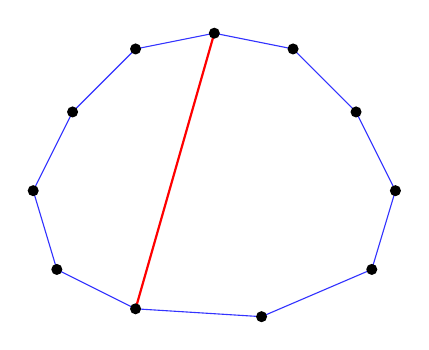
\begin{tikzpicture}
		% Define the vertices of the rounded irregular decagon
\coordinate (A) at (2, 0);
\coordinate (K) at (0.6, -0.6); % New vertex between A and J
\coordinate (J) at (-1, -0.5);
\coordinate (I) at (-2, 0);
\coordinate (H) at (-2.3, 1);
\coordinate (G) at (-1.8, 2);
\coordinate (F) at (-1, 2.8);
\coordinate (E) at (0, 3);
\coordinate (D) at (1, 2.8);
\coordinate (C) at (1.8, 2);
\coordinate (B) at (2.3, 1);

% Draw the polygon with the new vertex K
\draw[blue!80!white] (A) -- (K) -- (J) -- (I) -- (H) -- (G) -- (F) -- (E) -- (D) -- (C) -- (B) -- cycle;
\draw[thick, red] (E) -- (J);
% Draw a filled circle at each vertex with radius 1pt
\foreach \point in {A, B, C, D, E, F, G, H, I, J, K} {
	\fill (\point) circle (2pt);
}
	\end{tikzpicture}
\end{center}
	\end{wrapfigure}
	We will prove this using induction on number of sides of any convex polygon. For $n=3$ there is only one triangle. Hence the base case follows. Let this is true for $n=3,\dots, k-1$. For $n=k$ take any triangulation of the any polygon with $n$ sides. There is at least one edge among all the edges of all the triangles of the triangulation which is not a side of the polygon.  Let  $k_1$ be the number of vertices on the left side of the edge and $k_2$ be the  number of vertices on the right side of the edge.  
\end{adjustbox}\parinn

Then we have $k_1+k_2+2=k$. Now by induction the number of triangles in any triangulation of the $k_1+2$-polygon bounded by the edge and the $k_1$ vertices to the left is $k_1+2-2=k_1$. And the number of triangles in any triangulation of the $k_2+2$-polygon bounded by the edge and the $k_2$ vertices to the right of the edge is $k_2+2-2=k_2$. Hence the number of triangles in the triangulation of the $n$ sided polygon is $k_1+k_2=k-2$. Therefore by mathematical induction any triangulation of the convex polygon with $n$ sides has $n-2$ triangles.\parinn

Therefore any triangulation of a regular polygon with $n$ sides has $n-2$ triangles. 
\item 	We will count the number of triangulations for general convex polygon with $n$ sides. Suppose $T_n$ denote the number of triangulations of a $n$ sided convex polygon. We will find a recursion relation for $T_n$. 

\begin{adjustbox}{minipage={\linewidth}, valign=t}
	
	\begin{wrapfigure}{t}{0.4\linewidth}
		
		\begin{center}
			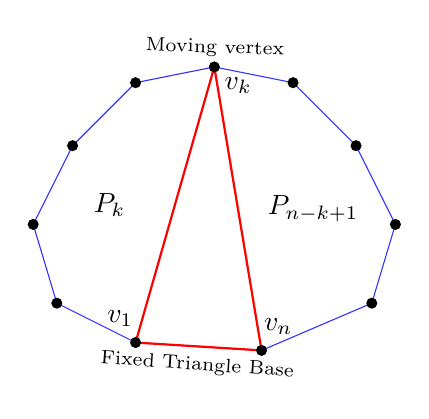
\begin{tikzpicture}
				% Define the vertices of the rounded irregular decagon
				\coordinate (A) at (2, 0);
				\coordinate (K) at (0.6, -0.6); % New vertex between A and J
				\coordinate (J) at (-1, -0.5);
				\coordinate (I) at (-2, 0);
				\coordinate (H) at (-2.3, 1);
				\coordinate (G) at (-1.8, 2);
				\coordinate (F) at (-1, 2.8);
				\coordinate (E) at (0, 3);
				\coordinate (D) at (1, 2.8);
				\coordinate (C) at (1.8, 2);
				\coordinate (B) at (2.3, 1);
				
				% Draw the polygon with the new vertex K
				\draw[blue!80!white] (A) -- (K) -- (J) -- (I) -- (H) -- (G) -- (F) -- (E) -- (D) -- (C) -- (B) -- cycle;
				\draw[thick, red] (E) node[above, rotate=-2, black]{\scriptsize{Moving vertex}} node[below right, black]{$v_k$}-- (J)  node[midway, left=0.5cm,black]{$P_{k}$}  node[above=3mm, left=-1mm, black]{$v_1$}-- (K) node[midway, below, black,rotate=-4]{\scriptsize{Fixed Triangle Base}} node[above=3mm, right=-1mm, black]{$v_n$} -- (E)  node[midway, right=0.25cm,black]{$P_{n-k+1}$};
				% Draw a filled circle at each vertex with radius 1pt
				\foreach \point in {A, B, C, D, E, F, G, H, I, J, K} {
					\fill (\point) circle (2pt);
				}
			\end{tikzpicture}
		\end{center}
	\end{wrapfigure}
\parinn

Let $P_n$ denote a polygon with $n$ sides. Now we first fix an edge. We index the vertices with $v_i$ for $i\in[n]$ anticlockwise where the fixed edge is between $v_1$ and $v_n$. For any triangulation of $P_n$ this edge becomes a base of a triangle for some triangle in any triangulation of $P_n$. For the triangle having the fixed edge we already chose 2 vertices and only the third vertex has to chosen. So there are in total $n-2$ choices to choose the third vertex of the triangle with the fixed edge as base. Let the third vertex be $k$. Hence $1<k<n$. Hence the triangle $\triangle v_1v_kv_n$ divides $P_n$ into two regions. On the right side of the $\ov{v_1v_k}$ edge there are $k-1$ vertices of $P_n$. Hence the vertices $v_1,v_2,\dots, v_k$ forms  forms a $k$ sided polygon $P_{k}$. And on the left side of the $\ov{v_kv_n}$ edge there are $n-k+1$ many vertices. Hence the vertices $v_n,v_{n-1},\cdots v_k$ forms a $n-k+1$ sided polygon $P_{n-k+1}$. 
\end{adjustbox}


Now $P_k$ can be triangulated in $T_k$ many ways and $P_{n-k+1}$ can be triangulated in $T_{n-k+1}$ many ways. Therefore in total for the current choice of $k$ there are $T_k\cdot T_{n-k+1}$ many triangulations of $P_n$. Now since $k$ can be the other vertex adjacent to $v_1$ or $v_n$ we will take $T_2=1$. This is because even though there is no polygon with $2$ vertices we $n-2+1\neq 0$ and therefore we can still count $T_{n-k+1}$ and multiply with $T_2$ to get the total number of triangulations when $k=2$. Similarly we we can count total number of triangulations when $n-k+1=2\implies k=n-1$. Therefore we have the following recursion relation $$T_n=\sum_{k=2}^{n-1}T_k\cdot T_{n-k+1}$$
\begin{lemma}
	$T_n=C_{n-2}$ for $n\geq 2$, $n\in\bbN$ where $C_n$ is the $n^{th}$ Catalan Number.
\end{lemma}
\begin{proof}
	We will show this using induction on $n$. For $n=2$ we have $T_2=1$ and we also know $C_0=1$. Hence the base case is followed. Let this is true for $n=2,\dots, k-1$. Now by the recursion relation we have$$T_k  = \sum_{m=2}^{k-1}T_m\cdot T_{k-m+1}  = \sum_{m=2}^{m-1}C_{m-2}\cdot C_{k-m+1-2} =\sum_{m=2}^{k-1}C_{m-2}\cdot C_{k-m-1} = \sum_{m=1}^{k-2}C_{m-1}\cdot C_{k-m-2}=C_{k-2}$$Therefore by Mathematical induction we have that $T_n=C_{n-2}$ for $n\geq 2$, $n\in\bbN$.
\end{proof}
Therefore number of triangulations of $n$-sided convex polygon is $C_{n-2}$ where $C_n$ is the $n^{th}$ Catalan Number. Since the given polygon is a regular $n$-sided polygon it is also a convex polygon. Therefore number of triangulations of a $n$-sided regular polygon is $C_{n-2}$.
	\end{itemize}

\item \begin{itemize}
	\item Suppose we have a regular polygon with $n$ sides. We label the vertices with $v_0,\dots, v_{n-1}$. Now any triangulation of the polygon has a triangle which has at least one edge which is a diagonal. Consider the diagonal $\ov{v_av_{a+k}}$, $n-2>k>2$. Such a diagonal divides the polygon into two parts. \parinn
	
	Consider the part with lesser number of vertices and if the two parts have same number of vertices then consider any one. So consider the polygon made of those vertices using the edges of the polygon and the diagonal. We will show a necessary and sufficient condition for which such a a polygon can be triangulated by isosceles. 
	
	\begin{lemma}\label{p5lm1}
		Let $n>3$. Consider the  polygon $D_t$ with vertices $v_0,\dots, v_t$ where the following are satisfied:\begin{enumerate}
			\item $|\ov{v_{i-1}v_i}|=|\ov{v_{j-1}v_j}|$ for any $i,j\in [t]$ 
			\item $|\ov{v_0v_n}|>|\ov{v_i,v_j}|$ for all $i,j\in\{0,\dots, t\}$, $j\geq i$ with the property $j-i\neq t$ 
			\item  $\angle v_{i-1}v_iv_{i+1}=\angle v_{j-1}v_jv_{j+1}$ for all $i,j\in[t-1]$
		\end{enumerate} then $D_t$ can be triangulated with isosceles triangles if and only if $n=2^k$ for some $k\in\bbN$, $k>1$.
	\end{lemma}
\begin{proof}
	We will first show that if $t=2^k$ then $D_t$ can be triangulated with isosceles triangles.We will prove this using induction on $k$. For base case let $k=2$. Then  consider the triangulation for $t=4$ with the triangles $\{\triangle v_0v_1v_2, \triangle v_0v_2v_4, \triangle v_2v_3v_4\}$. Hence the base case follows. Then the  second property basically says that $\ov{v_0v_t}$ is the biggest among the diagonals and sides of the polygon. This side then has to be a bases of an isosceles triangles. Since there are odd number of vertices we form the isosceles triangle $\triangle v_0v_{2^{k-1}}v_{2^k} $ since only $|\ov{v_0,v_{2^{k-1}}}|\neq |\ov{v_{2^{k-1}},v_t}|$ and $|\ov{v_0,v_i}|\neq |\ov{v_i,v_t}|$ for all $i\in[t-1]$ where $i\neq 2^{k-1}$. 
	
	\begin{figure}[h]
		\centering
		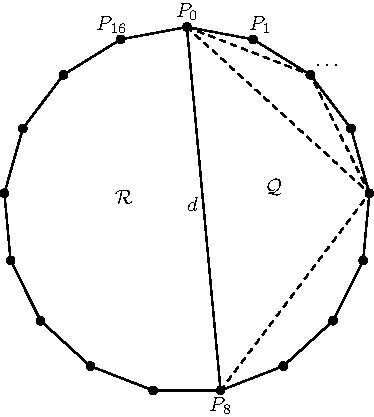
\includegraphics{workspace.pdf}
	\end{figure}

	Now we are left with 2 polygons. One is constructed by the vertices $v_0,\dots, v_{2^{k-1}}$ and the other one is constructed by the vertices $v_{2^{k-1}}, \dots, v_{2^{k}}$ Both of them satisfies the properties of the properties in the lemma. Hence each of them form a $D_{2^{k-1}}$, Therefore by inductive hypothesis they are  triangulated with isosceles triangles. Thus recursively we keep triangulating $D_{2^k}$ using isosceles triangles until we obtain a $D_1$ which is an isosceles triangle. Hence $D_{2^k}$ can be triangulated by isosceles triangles. Also observe that for $t=2^k$ there is only one possible triangulation of $D_t$ using isosceles triangles since at each step we have only one possible choice to construct the triangulation using isosceles triangles.
	
	We will show that $t=2^k$ is sufficient. First we will show $t$ is not odd.  Suppose $t$ is odd. Let $t=2k+1$. By the second property $\ov{v_0v_t}$ is the biggest among all diagonals and sides of the polygon. Therefore this edge has to be  the base of the isosceles triangles having the edge $\ov{v_0v_t}$. Since $t$ is odd the edge $\ov{v_{k}v_{k+1}}$ is parallel to the edge $\ov{v_0v_t}$. Therefore for all $i\in [t-1]$ we have $|\ov{v_0,v_i}|\neq |\ov{v_i,v_t}|$. Therefore there is not isosceles triangle which uses the vertices of $D_t$ and the edge $\ov{v_0v_t}$. But that is not possible if $D_t$ can be triangulated using isosceles triangles. Hence contradiction. Hence $t$ can not be odd. Therefore $t$ is even.
	
	Now we will show if $t$ is of the form $2^l(2k+1)$ where $k,l\in\bbN$ and $l,k\neq 0$, then also $D_t$ can not be triangulated using isosceles triangles. Again the edge $\ov{v_0,v_t}$ is the base of the isosceles triangle in any triangulation of $D_t$ using isosceles triangles. Now to construct an isosceles triangle using vertices of $D_t$ and edge $\ov{v_0,v_t}$ there is only one choice for the third vertex which is $2^{l-1}(2k+1)$ since otherwise for all $i\in [2^l(2k+1)]$, $i\neq 2^{l-1}(2k+1)$ we have $|\ov{v_0,v_i}|\neq |\ov{v_i,v_t}|$. So the $\triangle v_0v_{2^{l-1}(2k+1)}v_t$ is an isosceles triangles. Hence any triangulation of $D_t$ using isosceles triangles has the triangle $\triangle v_0v_{2^{l-1}(2k+1)}v_t$. Now the polygons constructed using $\{v_0,\dots, v_{2^{l-1}(2k+1)}\}$ and $\{v_{2^{l-1}(2k+1)},\dots, v_t\}$ follows the 3 properties given in the lemma. Hence they forms two $D_{{2^{l-1}(2k+1)}}$. Hence any triangulation of $D_t$ using isosceles triangles gives a triangulation of $D_{2^{l-1}(2k+1)}$ using isosceles triangles. If $l-1>0$ then again any triangulation of $D_{2^{l-1}(2k+1)}$ with isosceles triangles use the isosceles triangle $\triangle v_0 v_{2^{l-2}(2k+1)}v_{2^{l-1}(2k+1)}$. Again we get 2 polygons $D_{2^{l-2}(2k+1)}$. Therefore any triangulation  of $D_{2^{l-1}(2k+1)}$ using isosceles triangles gives a triangulation of $D_{2^{l-2}(2k+1)}$ using isosceles triangles. Hence any triangulation of $D_{2^l(2k+1)}$ using isosceles triangles gives a triangulation of $D_{2^{l-2}(2k+1)}$ using isosceles triangles. Continuing like this we get any triangulation of $D_{2^l(2k+1)}$ using isosceles triangles gives a triangulation of $D_{2k+1}$ using isosceles triangles. But we showed earlier that $D_{2k+1}$ can not have   a triangulation using isosceles triangles. Hence contradiction. Therefore if $n$ is of the form $2^l(2k+1)$ where $k,l\in\bbN$ and $k,l\neq 0$ then $D_t$ can not be triangulated using isosceles triangles.
	
	This leaves with only option fo $t$ to be of the form $2^k$ where $k\in \bbN$ and $k>1$. Hence $D_t$ can be triangulated using isosceles triangles where $t>3$ if and only if $t=2^k$ for some $k>1$, $k\in\bbN$.
\end{proof}

Suppose the regular polygon with vertices $v_0,\dots, v_{n-1}$ can be triangulated using isosceles triangles. If $n=3$ then it is a equilateral triangle hence it can be triangulated using isosceles triangles. If $n=4$ then it is a square. Therefore if we take any diagonal then it divides the square into two isosceles triangles. Therefore for $n=4$ also we can triangulate into isosceles triangles.

Now consider $n>4$. Take any triangulation of the polygon using isosceles triangles. Then take  any triangle consisting of at least 2 diagonals of the polygon. Without loss of generality we can think the edge is $\ov{v_0,v_l}$ and the other vertex is $v_k$ where $1<k<l-1$ and $\lt\lfloor\frac{n}2\rt\rfloor\leq l< n$. Now since $\triangle v_0v_lv_k$ is isosceles we have $k=\frac{l}2$. Now the vertices $v_0,\dots  v_k$ forms $D_{k}$ defined in \lemref{p5lm1}. Similarly the vertices $v_k,\dots, v_l$ also forms $D_k$. Since $k>2$ by \lemref{p5lm1} we know $k=2^m$ for some $m>1$, $m\in\bbN$.  Now we will see case wise for $l$:\begin{itemize}
	\item \textbf{Case 1:} $l=n-1$. Then we have in the two $D_k$ we counted the vertex $v_k$ each time once. The total number of vertices in the polygon is $n$ and each $D_k$ has $k+1$ many vertices. Therefore So we have $$n=2\times (2^m+1)-1\implies 2^{m+1}+1$$
	\item \textbf{Case 2:} $l=n-2$. Then the triangle $\triangle v_0v_{n-1}v_{n-2}$ is isosceles. In the two $D_k$ we counted the vertex $v_k$ each time once and we didn't counted the vertex $v_{n-1}$. Therefore we have $$n-1=2(2^m+1)-1\implies n=2^{m+1}+2$$
	\item \textbf{Case 3:} $l<n-2$. Then the vertices $v_0,\dots, v_l$ form a $D_l$. That means $D_l$ is triangulated using isosceles triangles. Therefore using \lemref{p5lm1} we have $l=2^p$ for some $p\in\bbN$, $p>1$. Then we have $$n+3=2(2^m+1)+(2^p+1)\implies n=2^{m+1}+2^p$$
\end{itemize}
Hence $n$ has the form $2^{m+1}+2^p$ for some $m,p\bbN\cup \{0\}$. the $n=3$ and $n=4$ case also comes under this form for $m=p=0$ and $m=p-1=0$ respectively. Hence for any $n$ the regular polygon using the vertices $v_0,\dots, v_n$ can be triangulated using isosceles triangles if $n=2$ or $n=2^{m+1}+2^p$ for some $m,p\in\bbN\cup\{0\}$.

Now we will show triangulation for $n=2^{m+1}+2^p$ with isosceles triangles. We can always assume $m+1\geq p$ without loss of generality. Then $n=2^{m+1}+2^p=2^P(2^{m+1-p}+1)$. So we will show first that for $n=2^k+1$ we can triangulate using isosceles triangles and then we will show if for any $n$ we can triangulate using isosceles triangles then we can also triangulate $2n$ using isosceles triangles. 
\begin{lemma}\label{p5lm3}
	All regular polygons with $n = 2^k + 1$ or $n=4$ have triangulations with isosceles triangles.
\end{lemma}
\begin{proof}
	For $n=4$ we take the triangles $\{\triangle v_0v_1v_2, \triangle v_0v_2v_4, \triangle v_2v_3v_4\}$. This is a triangulation for $n=4$ using isosceles triangles. For $n=2^k+1$ we take the triangle $\triangle v_0v_{2^{k-1}}v_{2^{k}}$. Now the vertices $v_0,\dots, v_{2^{k-1}}$ forms $D_{2^{k-1}}$ and the vertices $v_{2^{k-1}},\dots, v_{2^k}$ also forms $D_{2^{k-1}}$. We have shown in \lemref{p5lm1} how to triangulate $D_{2^{k-1}}$ using isosceles triangles. Therefore we have the lemma.
\end{proof}
\begin{lemma}\label{p5lm4}
	 If a regular polygon with $n$ sides has a  triangulation with isosceles triangles, then the regular polygon with $2n$ sides also has a triangulation with isosceles triangles. 
\end{lemma}
\begin{proof}
	We have the vertices $v_0,\dots, v_{2n-1}$. We construct the diagonals $\ov{v_{2i-2}v_{2i}}$ for $i\in [n]$ where $v_{2n}\coloneq v_0$. Now the triangles $\triangle v_{2i-2}v_{2i-1}v_{2i}$ for all $i\in [n]$ is isosceles triangle. Also the polygon we vertices $v_0,v_{2},v_4,\dots, v_{2i},\dots, v_{2n-2}$ where $0\leq i\leq n-1$ forms a regular polygon with $n$ sides. And we know a  regular polygon with $n$ sides has a  triangulation with isosceles triangles. Hence this gives a triangulation of regular polygon with $2n$ sides using isosceles triangles. 
\end{proof}
Therefore we can have a triangulation of a regular polygon with $n$ sides using isosceles triangles if and only if $n$ is of the form $n=2^{m+1}+2^p$ where $m,p\in\bbN\cup\{0\}$.
\item We will now consider all the triangulations which are same upon rotation to be same. Hence all the triangulations which are same under rotation contributes only 1 in total to the count. We claim that there is only 1 triangulation using isosceles triangles. From the previous part we know for $n$ of the form $n=2^{m+1}+2^p$ there is a triangulation of the regular polygon with $n$ sides using isosceles triangles. WLOG we can assume $m+1\geq p$. Therefore $n=2^{m+1}+2^p=2^p(2^{m+1-p}+1)=2^p(2^q+1)$ where $q=m+1-p\geq 0$\parinn

We will also proceed like we did in the previous part. Any triangulation of the regular polygon with $n$ sides using isosceles triangles has a triangle which has at least 2 sides which are diagonals of the polygon. We can relabel the vertices by rotating them so that we can say the triangle is $\triangle v_0v_lv_k$ where $\lt\lfloor\frac{n}2\rt\rfloor\leq l<n$ and $1<k<l-1$ and since the triangle is isosceles we have $k=\frac{l}2$. Then the vertices $v_0,\dots  v_k$ forms $D_{k}$ and similarly the vertices  $v_k,\dots, v_l$ also forms $D_k$. Now we have $k\geq 2$. Hence by \lemref{p5lm1} we have $k=2^s$ for some $s\in\bbN$, $s\geq 1$. We have scene in the proof of \lemref{p5lm1} that $D_k$ can be triangulated in an unique way using isosceles triangles.  

That leaves us the polygon formed with the vertices $v_0,\dots, v_l$. If $l=n-1$ then it is just an edge. In that case for such triangulation $n+1$ can be written as twice of a number of the form $2^s+1$ since $D_k$ has $k+1$ many vertices since we are counting $v_k$ two times in total once in each $D_k$. For this case is only possible when $n=2^{s+1}+1$. Conversely we can say if $n$ is of the form $n=2^{s+1}+1$ then we get $k=2^s$ uniquely. 

If $l<n-1$ the $v_0,\dots, v_l$ forms $D_l$. In order to $D_l$ have triangulation using isosceles triangles $l$ has to be of the form $2^t+1$ where $t=\geq 1$ and $t\in\bbN$. Therefore in this case we count both $v_0$ and $v_l$ two times, once in each $D_k$ and $D_l$. So $n+3$ can be written in the form $2(2^s+1)+(2^t+1)=2^{s+1}+2^t +3\implies n=2^{s+1}+2^t$. Since $s,t\geq 1$ we have $n\geq 6$.  If $n$ is a sum of two powers of $2$ then $n$ there exists unique $s,t$ such that $n=2^s+2^t$ where $s,t\geq 1$ and $s,t\in\bbN\cup\{0\}$. Hence conversely if $n$ is of the form $n=2^s+2^t$ then from this we can say $k=2^{s-1}$ and $l=2^t$ uniquely and the triangle obtained divides the regular polygon into two $D_{2^{s-1}}$ and one $D_{2^t}$. 

Therefore for all $n$ of the form $n=2^{m+1}+2^p$ there is a unique triangulation of the regular polygon with $n$ sides using isosceles triangles.

So now removing the assumption that we take all the triangulations to be same which are same under rotation we obtain $n$ triangulations of the regular polygon using isosceles triangles. 
\end{itemize}
\end{itemize}
}


\end{document}
